%追加すべき事項
% - ? lossの図と説明
% - ? 追加実験
\chapter{実験}
\myaddchaplof{実験}

本章では、提案手法と実験方法の説明を行った後、実験結果の考察を行う。

\section{提案手法}

本節では、提案手法の説明を行う。

\subsection{提案手法の目標}
\label{sec:pr_purpose}

提案手法の目標は、Pix2pixを参考に作成した提案モデルを用いて音の高さと大きさを維持したままでギターの単音からハープの単音への音色の変換を行うことである。ここで、ある楽器を用いてある高さの一音を鳴らした時に出力される音として単音を定義する。また、音色の変換対象にギターとハープを選んだ理由は、弦楽器という共通点を持ちながらも音波の観察と音の聴き取りの評価により十分に異なると判定できると考えたからである。

\subsection{提案モデルの構造}
\label{sec:proposed}

提案モデルのGANには生成モデルと識別モデルのいずれにも変換元のギターの音を条件として与える~(\prettyref{fig:pr_model})~。基本構造はPix2pixと変わらないが、決定論的に音を生成するためにノイズを表すDropout層を使用していない点に注意が必要である。

また、44100~Hzのサンプリング周波数でサンプリングした1秒の音響信号を音のデータとして使用する。ここで、量子化ビット数が16ビットでチャンネル数が1であるため、この音のデータは44100の長さを持つ16ビット整数の一次元配列である。

\begin{figure}[b]
\centering
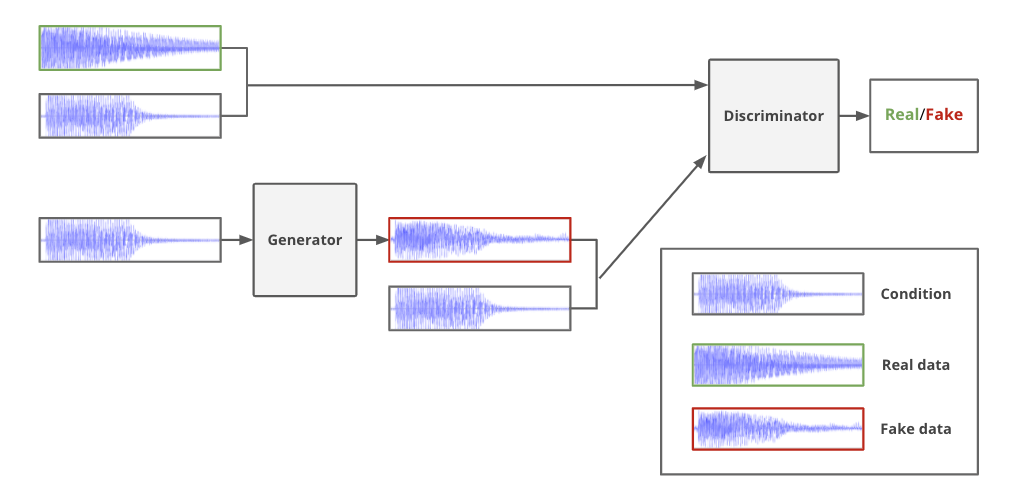
\includegraphics[width=0.9\columnwidth]{figure/pr_model.png}
\caption{提案モデルの全体図}
\label{fig:pr_model}
\end{figure}

%ここで改ページ
\clearpage

\subsection{生成モデルと識別モデル}

提案モデルの生成モデルと識別モデルを\prettyref{fig:pr}に示す。まず、灰色の箱は特徴量マップを表す。箱の上側と左側にそれぞれチャンネル数と特徴量マップとなる一次元配列の長さを示す。そして、矢印はニューラルネットワークの層の操作を表す。畳み込み層と逆畳み込み層では~(カーネルサイズ、パディング数、ストライド)~としてそれぞれの値を示し、活性化関数のLeakeyReLUでは負の実数の定義域での一次関数の傾きの値を示す。また、スキップコネクションではEncode時の特徴量マップをDecode時にも利用することで実装している。

\begin{figure}[b]
\centering
\begin{minipage}[b]{0.6\columnwidth}
\centering
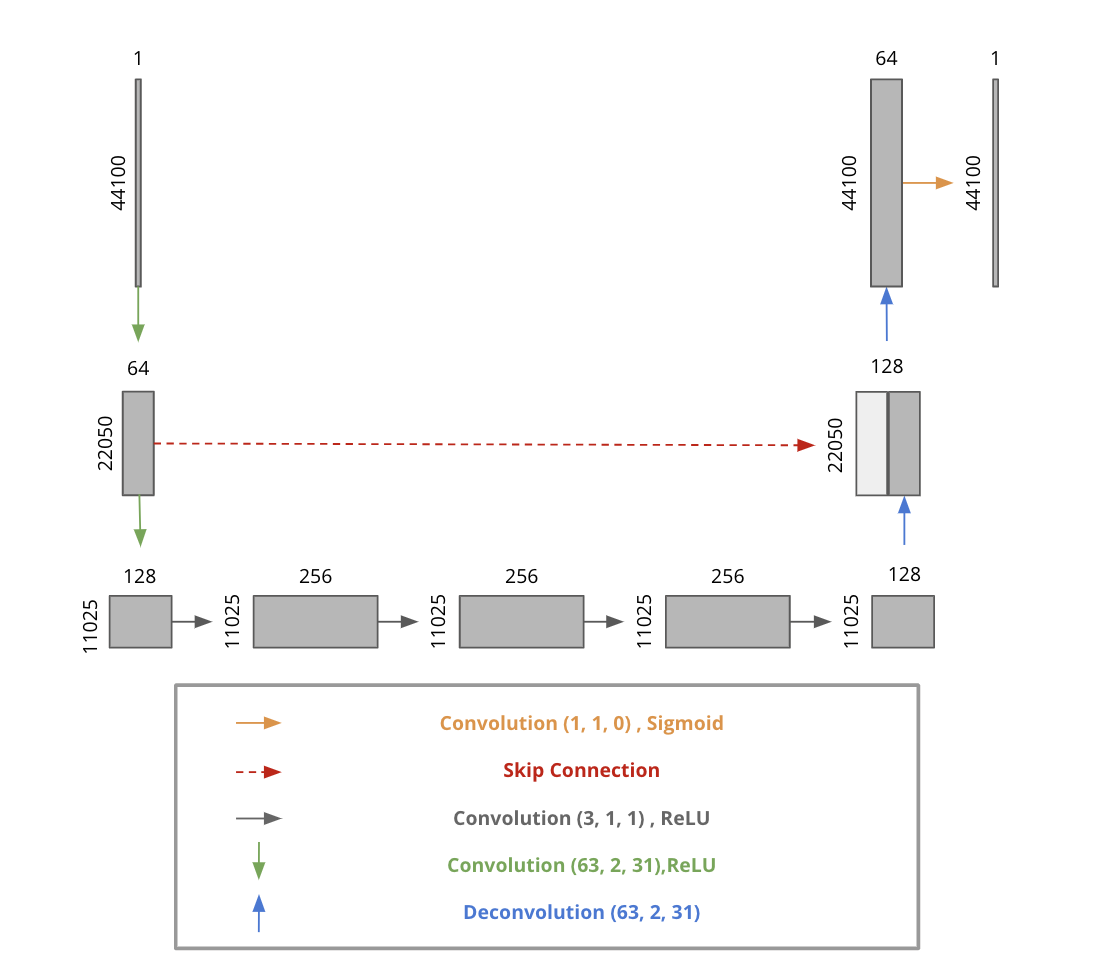
\includegraphics[width=\columnwidth]{figure/pr_generator.png}
\subcaption[本研究の生成モデル]{生成モデルのネットワーク}
\label{fig:pr_gen}
\end{minipage}\\
\begin{minipage}[b]{0.6\columnwidth}
\centering
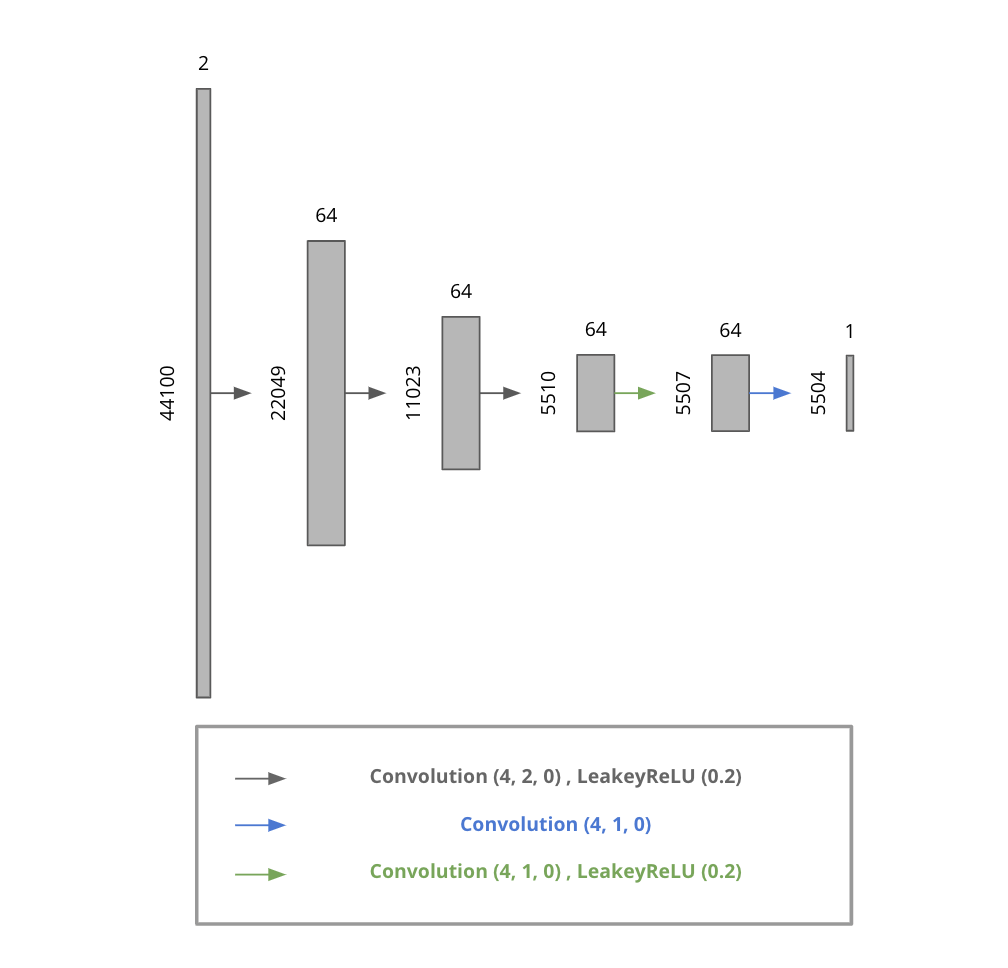
\includegraphics[width=\columnwidth]{figure/pr_discriminator.png}
\subcaption[本研究の識別モデル]{識別モデルのネットワーク}
\label{fig:pr_dis}
\end{minipage}
\caption{本研究の生成モデルと識別モデル}
\label{fig:pr}
\end{figure}

%ここで改ページ
\clearpage

\section{実験方法}

本節では実験方法の説明を行う。また、実験時のパラメータについては\prettyref{app:params}に示す。

\subsection{データセット}

データセットとして1秒のギターとハープの音を88組用いた。また、この88音は音の大きさが等しいものと仮定した。そして、音の高さとしてはA0$\sim$C8の88音の半音を選んだ。これらは一般的な88鍵のピアノのそれぞれの鍵盤の音に対応する~(\prettyref{fig:piano})~。

\subsubsection{音階表記}

本実験では西洋音楽の12音階表記を音階表記に用いる。この表記では、$C,C^{\sharp},D,D^{\sharp},E,F,F^{\sharp},G,$\\
$G^{\sharp},A,A^{\sharp},B$の12段階の音の高さの集合をオクターブとして定める。そして、それぞれのオクターブに番号を振り、440~Hzの音をA4と定めることで音の高さの絶対的な表記を可能にしている。

\begin{figure}[b]
\centering
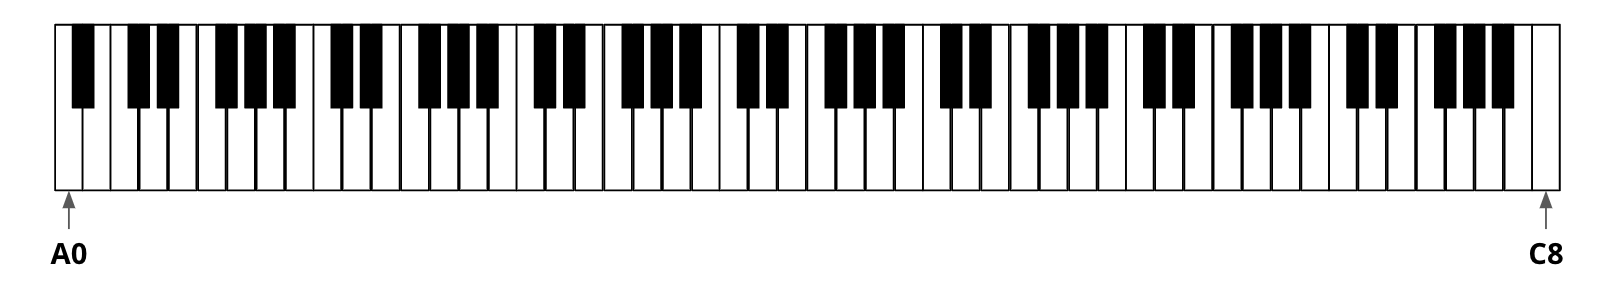
\includegraphics[width=0.8\columnwidth]{figure/piano.png}
\caption{88鍵のピアノの鍵盤}
\label{fig:piano}
\end{figure}

\subsection{実験1:提案モデルの表現力の評価実験}

88音を学習データと評価データのいずれでも使用し、同じ高さの音の間での変換をすることで、提案モデルの表現力を評価する実験を行った。

\subsection{実験2:提案モデルの汎化能力の評価実験}

88音のうち3/4を学習データ、1/4を評価データとする4分割交差検定をすることで、提案モデルの汎化能力を評価する実験を行った。また、この際のデータセットの分割方法を\prettyref{app:split}に示す。

\subsection{データ拡張}

88音と小さいサイズのデータセットへの過学習を防ぐため、振幅方向でのデータ拡張を行った。具体的には、各エポックの任意の学習データの振幅に一様乱数に従って$0.3\sim1.0$の乱数をかけた。

\subsection{評価方法}

\prettyref{sec:pr_purpose}の提案手法の目標を満たすかという観点から音波の観察と音の聴き取りにより評価を行った。また、データセットで組となる音の高さ~(基音)~は等しいが、基音より高い音~(上音)~の成分の組み合わせが異なるために音色の違いが生まれる。したがって、\prettyref{sec:result}では上音に注目した考察を中心に行う。

%ここで改ページ
\clearpage

\section{実験結果}
\label{sec:result}

実験結果の考察を本節では行う。また、実験結果として記載する波形の図は三つの波形を上から並べている。これらは上から順に、変換元のギターの波形、生成モデルの出力の波形、変換先のハープの波形、である。そして、本節には一部の音波のみを記載し、\prettyref{app:result}に実験結果の音波を全て記載する。

\subsection{実験1:提案モデルの表現力の評価実験}

提案モデルの表現力の評価実験を行ったところ、実験結果は二つに大別された。

\subsubsection{ハープの音を表現できた場合}

88音のうち86音ではハープの音を表現できた~(\prettyref{fig:88_88_good1})~。また、特にC4からD5$\sharp$の16音では目標のハープの音に極めて近い音色の音を生成できた~(\prettyref{fig:88_88_good2})~。これらの音は上音が少ないため、他の音と比べて表現が容易であったと考えられる。

\begin{figure}[b]
\centering
\begin{minipage}[b]{0.48\columnwidth}
\centering
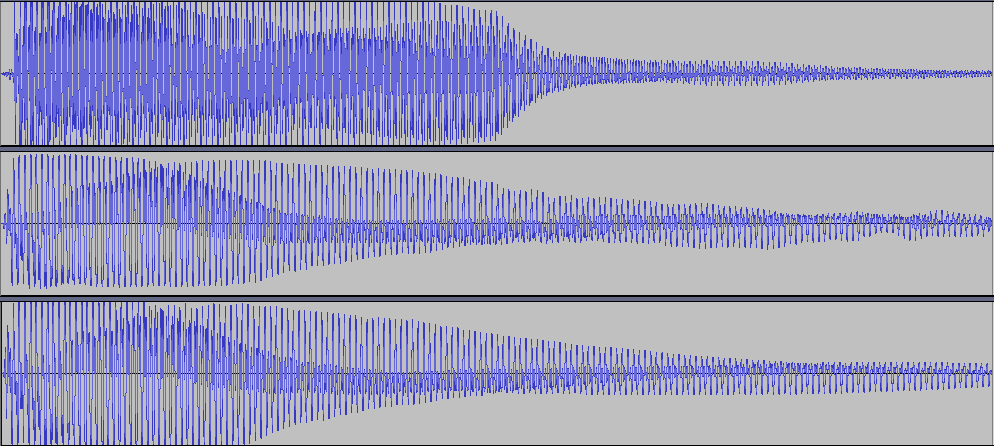
\includegraphics[height=90pt]{figure/88_88/f3.png}
\subcaption[F3の音波]{F3の0.000秒から1.000秒まで}
\label{fig:88_88_good1}
\end{minipage}
\begin{minipage}[b]{0.48\columnwidth}
\centering
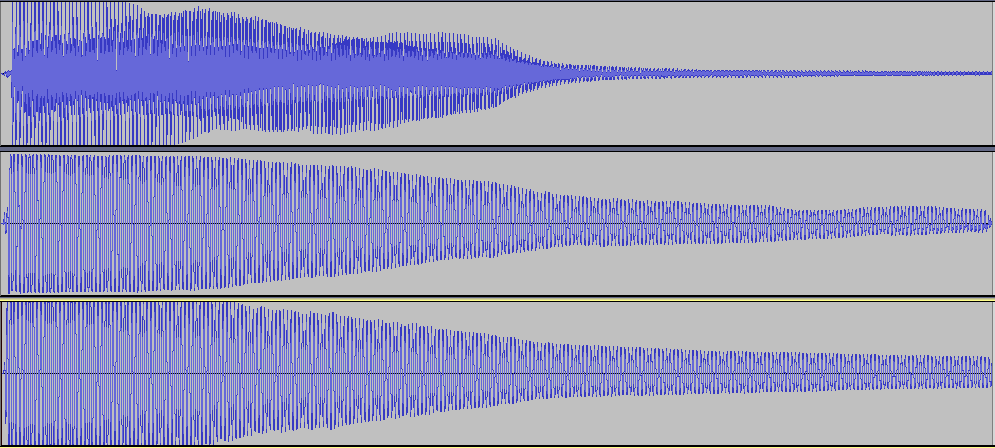
\includegraphics[height=90pt]{figure/88_88/c4.png}
\subcaption[C4の音波]{C4の0.000秒から1.000秒まで}
\label{fig:88_88_good2}
\end{minipage}
\caption[実験1:ハープの音を表現できた音波]{}
\end{figure}

\subsubsection{ハープの音を表現できなかった場合}
\label{sec:harp_rep}

D7$\sharp$とE7の2音では音の高さを維持できたが、ハープの音を十分に表現できなかった~(\prettyref{fig:88_88_bad})~。いずれの音でも学習データである変換先のハープの音の振動が安定しておらず、この不安定さを学習できなかった。また、高音では不安定な振動の学習データが多く、高音での安定したデータセットの作成が難しいことがわかった。

\begin{figure}[b]
\centering
\begin{minipage}[b]{0.48\columnwidth}
\centering
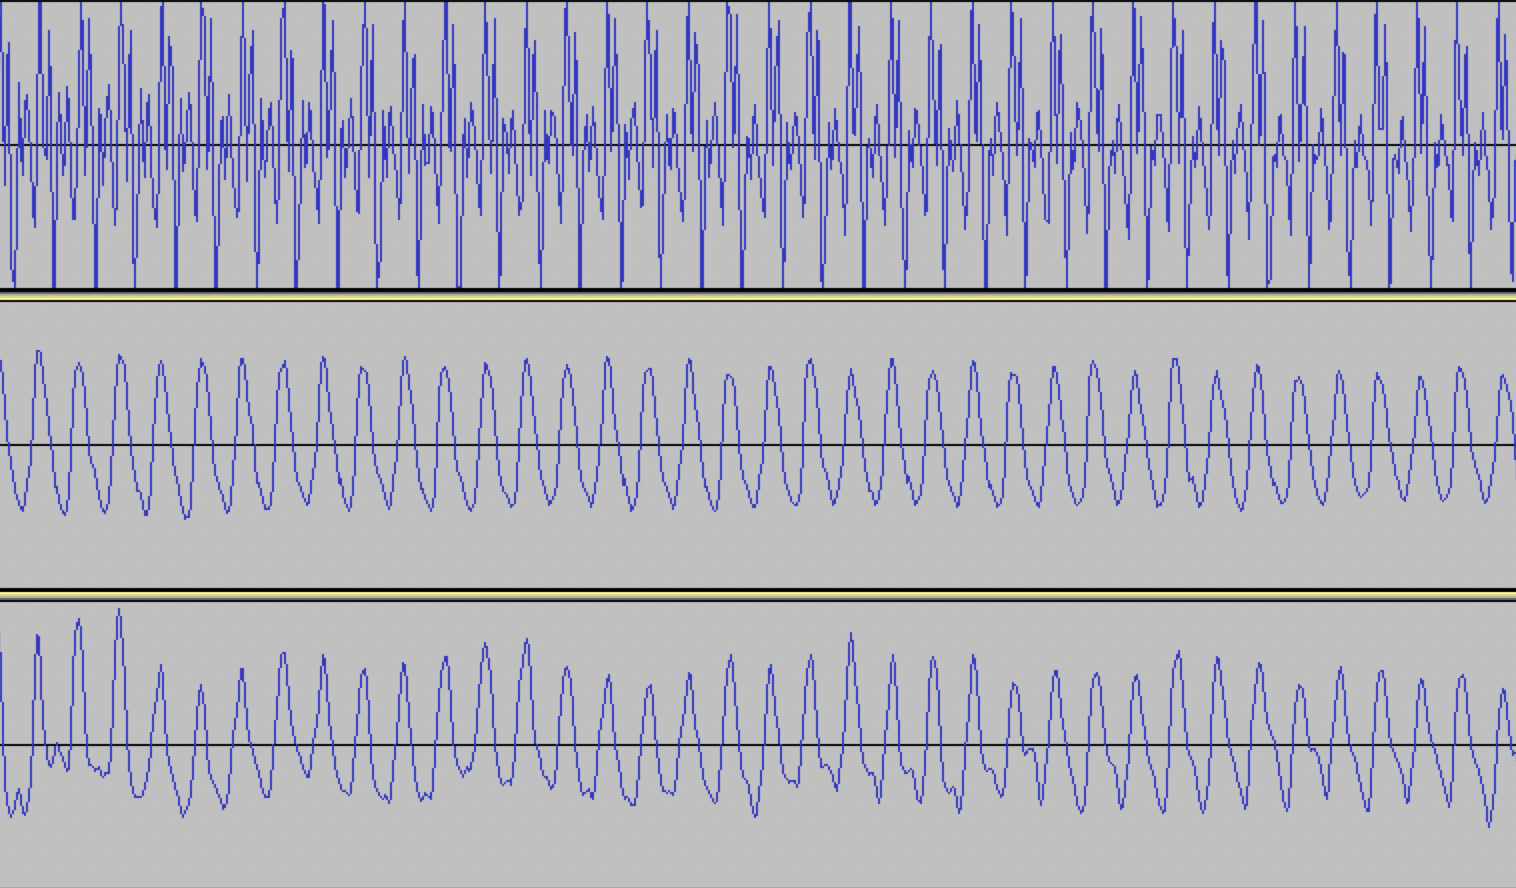
\includegraphics[height=90pt]{figure/88_88_det/d7s_0550_0700.png}
\subcaption[D7$\sharp$の音波]{D7$\sharp$の0.055秒から0.070秒まで}
\label{fig:88_88_bad1}
\end{minipage}
\begin{minipage}[b]{0.48\columnwidth}
\centering
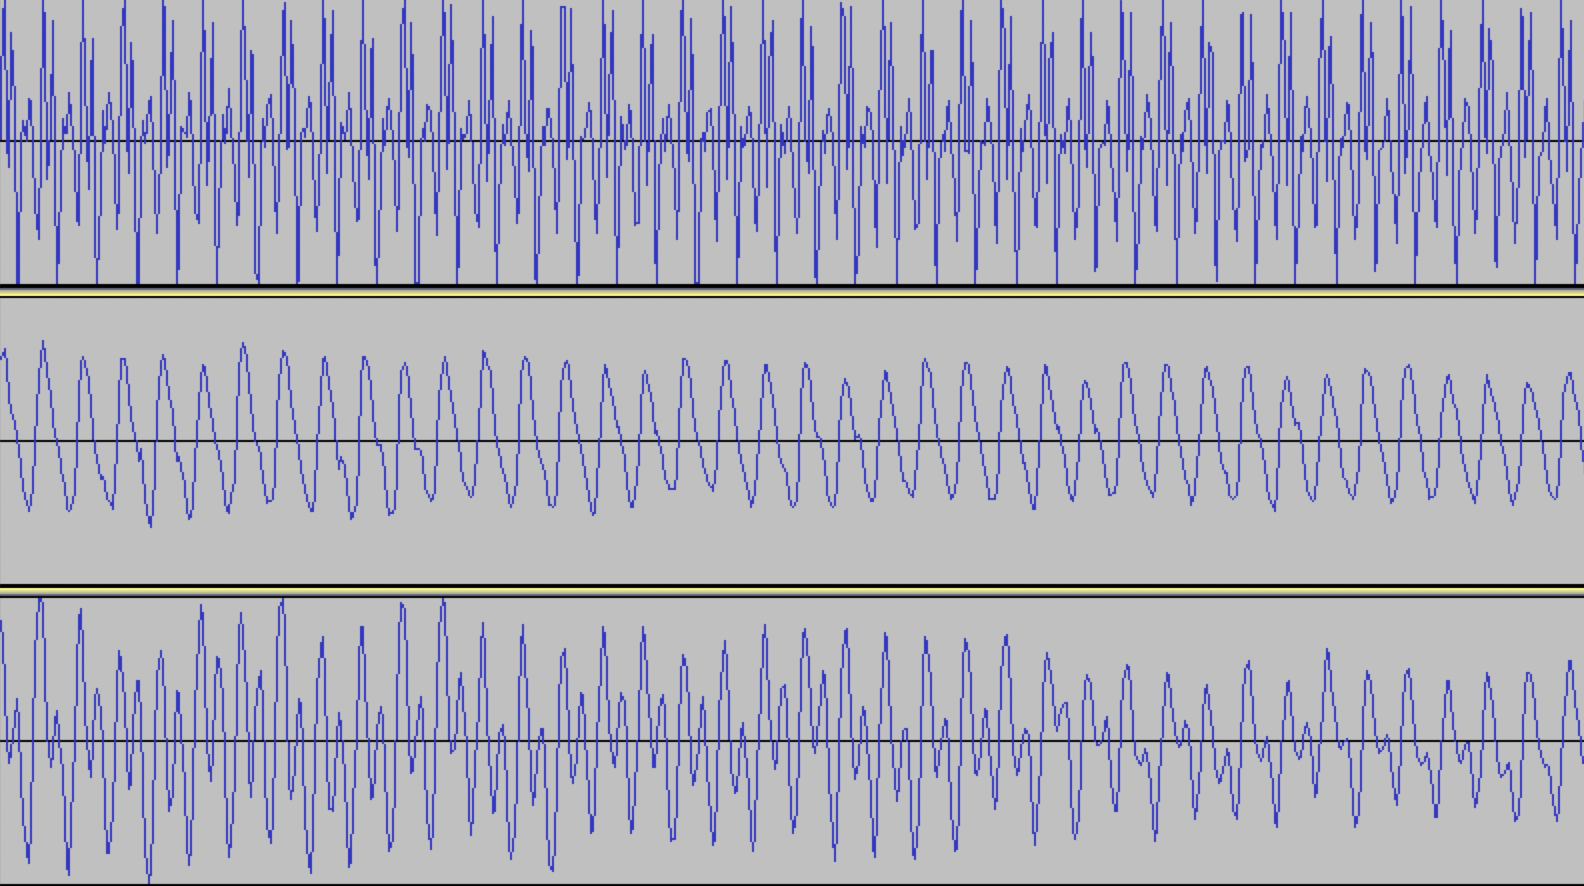
\includegraphics[height=90pt]{figure/88_88_det/e7_0550_0700.png}
\subcaption[E7の音波]{E7の0.055秒から0.070秒まで}
\label{fig:88_88_bad2}
\end{minipage}
\caption[実験1:ハープの音を表現できなかった音波]{}
\label{fig:88_88_bad}
\end{figure}

\subsection{実験2:提案モデルの汎化能力の評価実験}

提案モデルの汎化能力の評価実験を行ったところ、実験結果は三つに大別された。

\clearpage

\subsubsection{ハープの音を表現できた場合}

D4,D4$\sharp$,G4,F5,F5$\sharp$の5音ではハープの音を表現できた~(\prettyref{fig:66_22_near})~。これらの高さの音では提案モデルの表現力の評価実験の際にも特にハープの音色に近い音を生成でき、上音が少ないほど表現が容易であるという推察が強められた。

\subsubsection{ハープの音を表現できず音の高さも維持できなかった場合}

C7,D7$\sharp$,E7,F7$\sharp$,G7,G7$\sharp$,A7,B7,C8の9音では音の高さも維持できず、騒音が生成された~(\prettyref{fig:66_22_bad4})~。これらの高さの音では提案モデルの表現力の評価実験の際にもハープの音を表現できず、高音域における安定したデータセットの作成が難しいという推察が強められた。

\begin{figure}[t]
\centering
\begin{minipage}[b]{0.48\columnwidth}
\centering
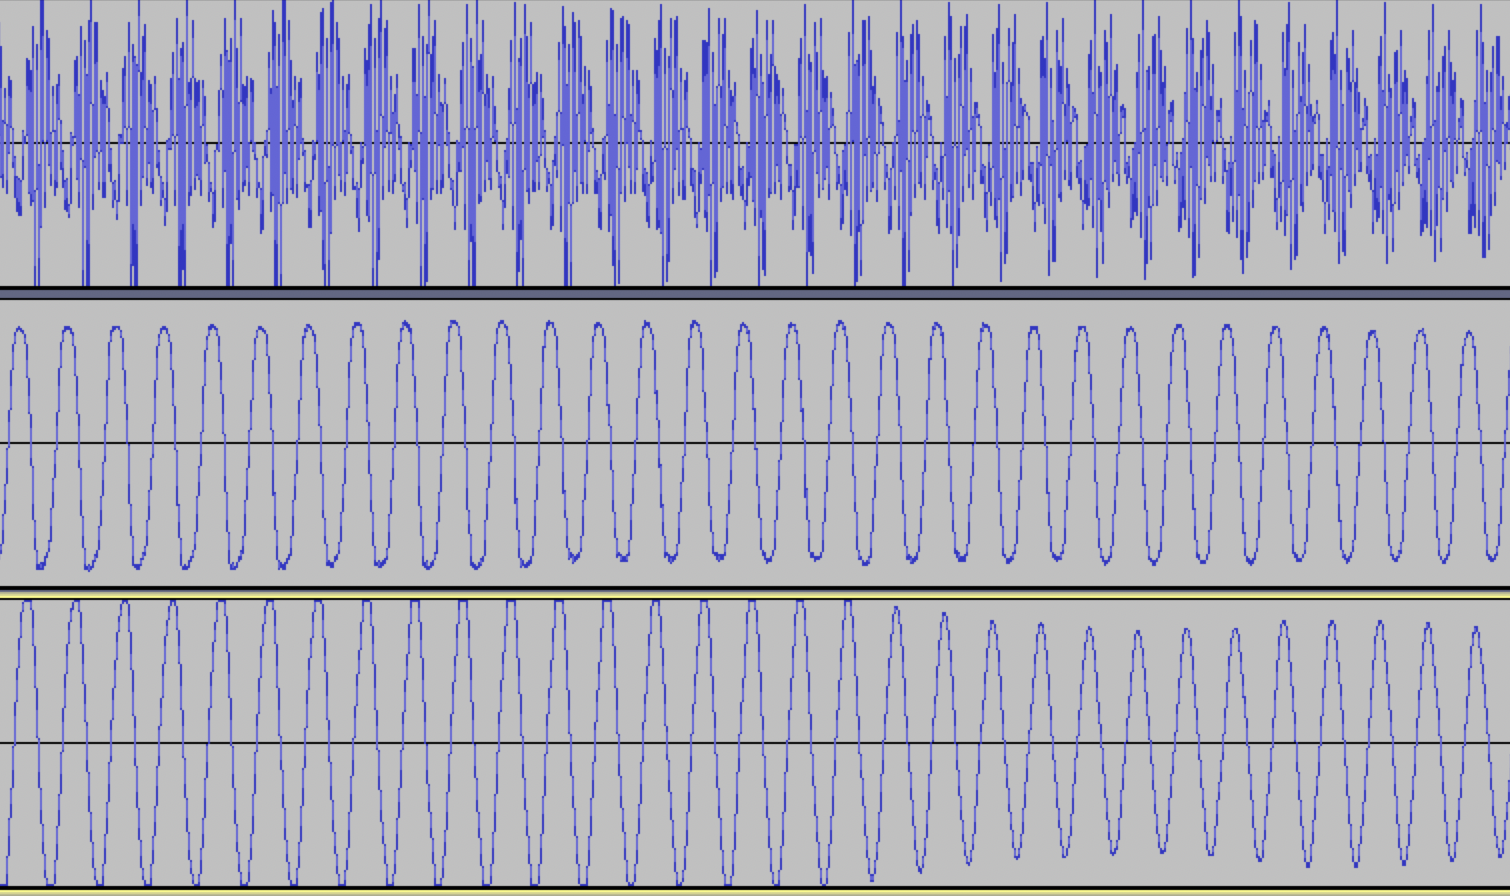
\includegraphics[height=90pt]{figure/66_22_det/d4s_0100_0200.png}
\caption[実験2:ハープの音を表現できた音波]{D4$\sharp$の0.100秒から0.200秒まで}
\label{fig:66_22_near}
\end{minipage}
\begin{minipage}[b]{0.48\columnwidth}
\centering
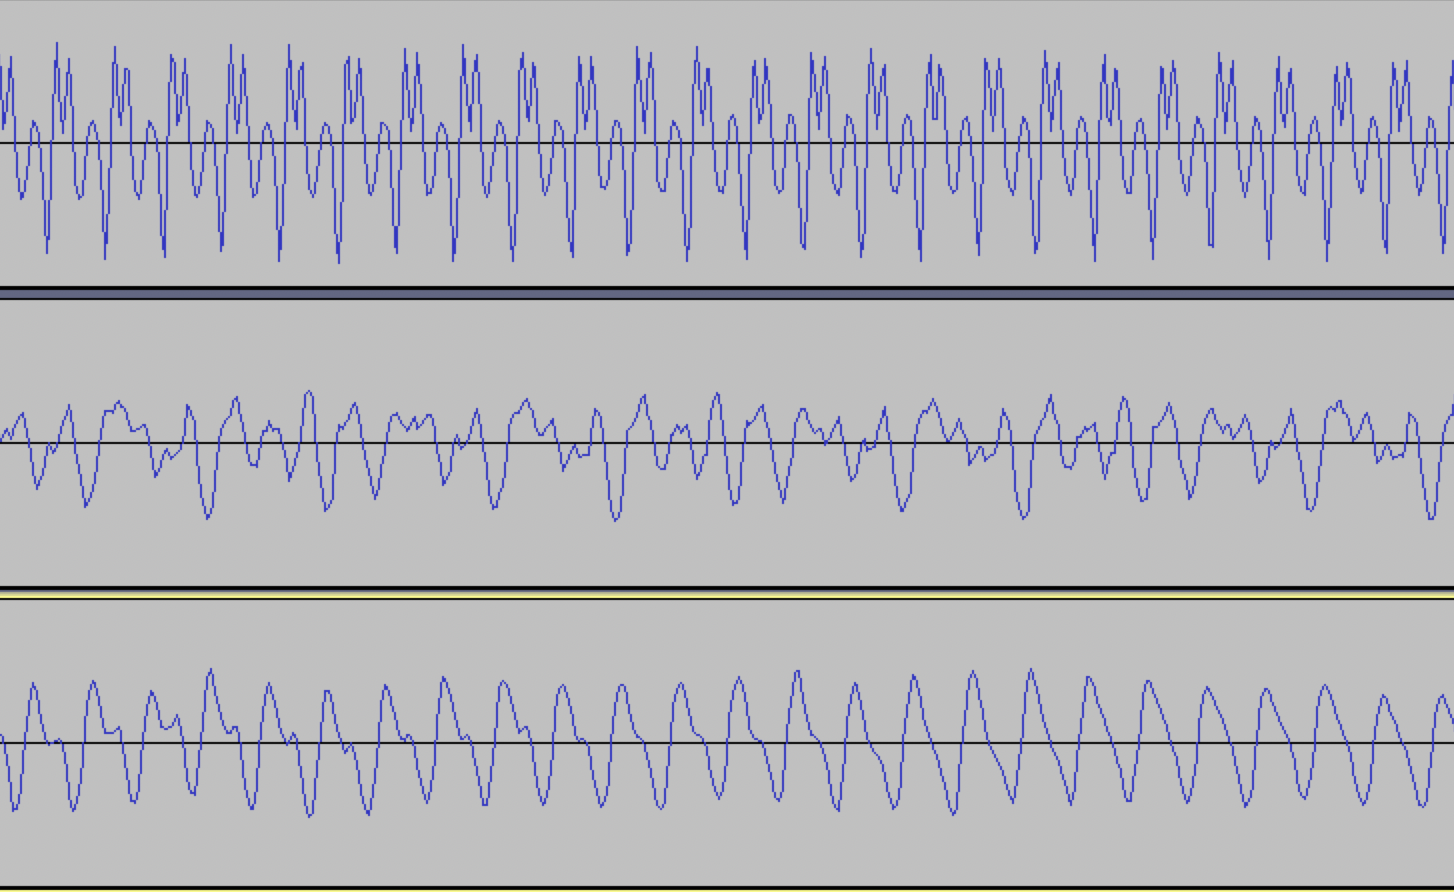
\includegraphics[height=90pt]{figure/66_22_det/d7s_0100_0110.png}
\caption[実験2:ハープの音を表現できず音の高さも維持できなかった音波]{D7$\sharp$の0.1700秒から0.110秒まで}
\label{fig:66_22_bad4}
\end{minipage}
\end{figure}

\subsubsection{ハープの音を表現できず音の高さを維持できた場合}

14音を除く74音では音の高さは維持できたがハープの音を表現できなかった~(\prettyref{fig:66_22_bad})~。これらの高さの音では生成された音波が安定した振動をせず上音の成分がハープよりも多い音波が多く観測された。また、これらの高さの音では提案モデルの表現力の評価実験の際にはハープの音色の音波を表現できていたため、提案モデルの汎化能力の低さが明らかになった。

\begin{figure}[b]
\centering
\begin{minipage}[b]{0.48\columnwidth}
\centering
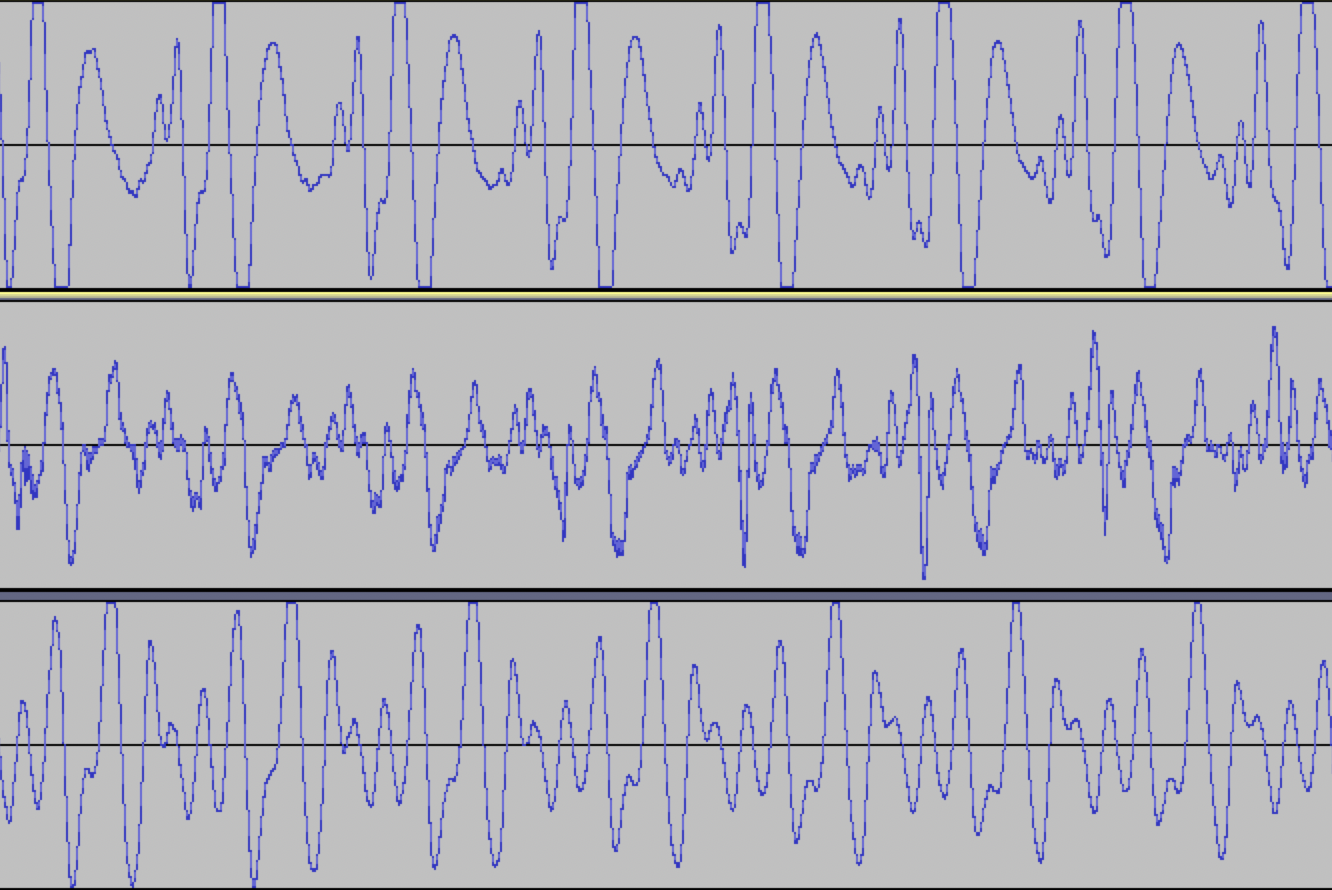
\includegraphics[height=90pt]{figure/66_22_det/d1_0300_0500.png}
\subcaption[D1の音波]{D1の0.300秒から0.500秒まで}
\label{fig:66_22_bad1}
\end{minipage}
\begin{minipage}[b]{0.48\columnwidth}
\centering
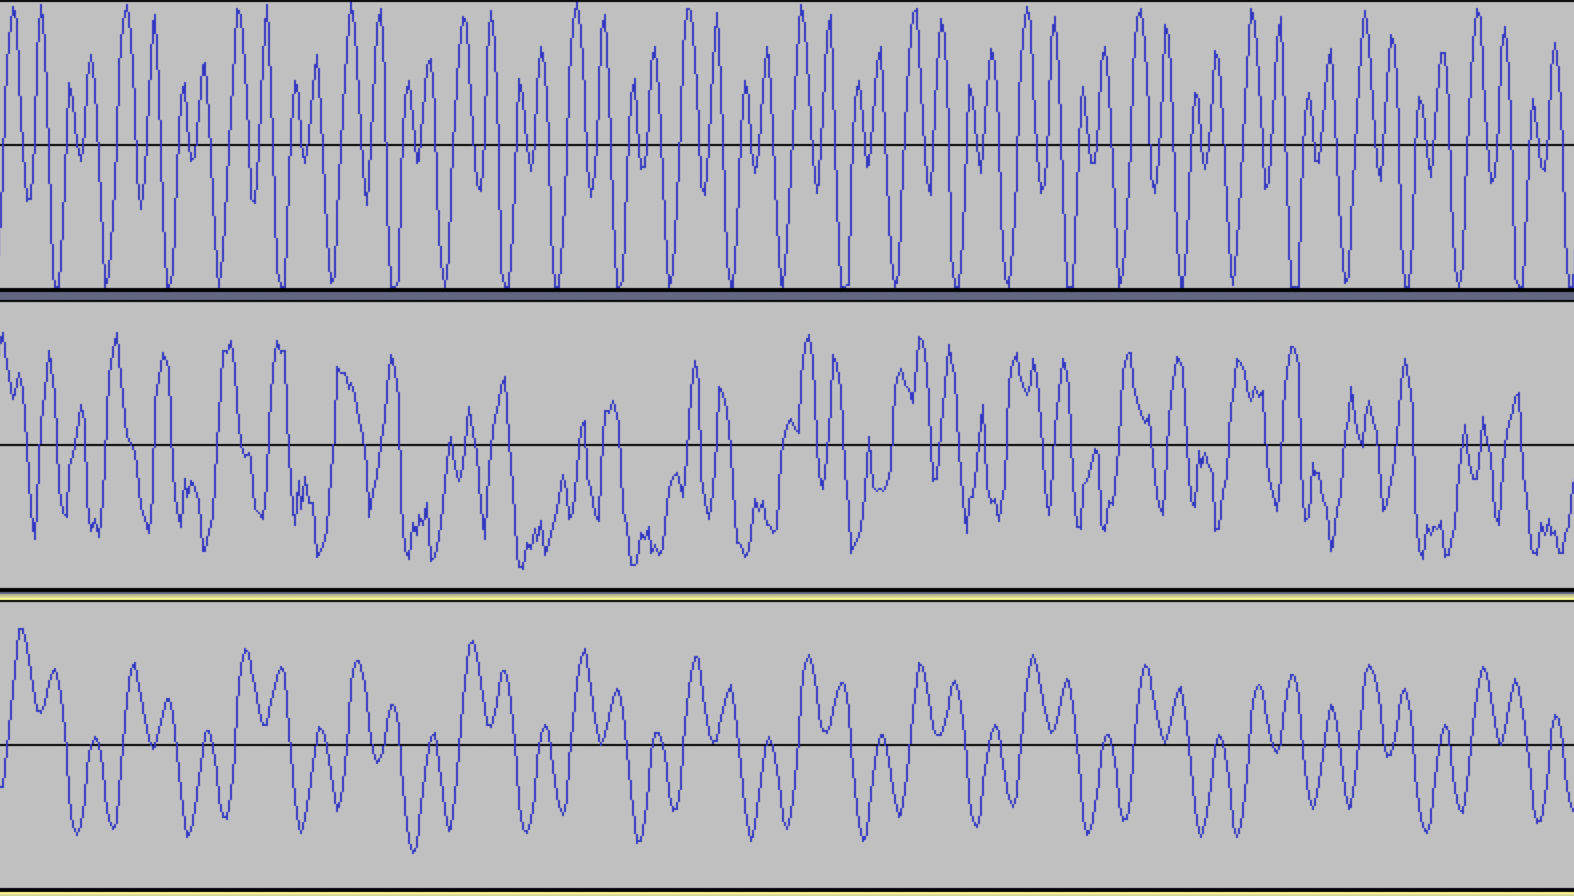
\includegraphics[height=90pt]{figure/66_22_det/f6_0070_0080.png}
\subcaption[F6の音波]{F6の0.070秒から0.080秒まで}
\label{fig:66_22_bad2}
\end{minipage}
\caption[実験2:ハープの音を表現できず音の高さを維持できた音波]{}
\label{fig:66_22_bad}
\end{figure}

\subsection{課題}

提案モデルの表現力の評価実験の実験結果からさらに四つの課題が明らかになった。

\subsubsection{音の減衰の表現}

振動の減衰を表現できていない音がいくつかあった。これらの音は、E2以下の低音域ではハープとは全く異なる波形で減衰し~(\prettyref{fig:88_88_reduce1})~、A6以上の高音域ではほとんど振動が見られなかった~(\prettyref{fig:88_88_reduce2})~。また、提案モデルの表現力不足で微小な振動の表現が難しいことが原因として考えられる。

\clearpage

\begin{figure}[t]
\centering
\begin{minipage}[b]{0.48\columnwidth}
\centering
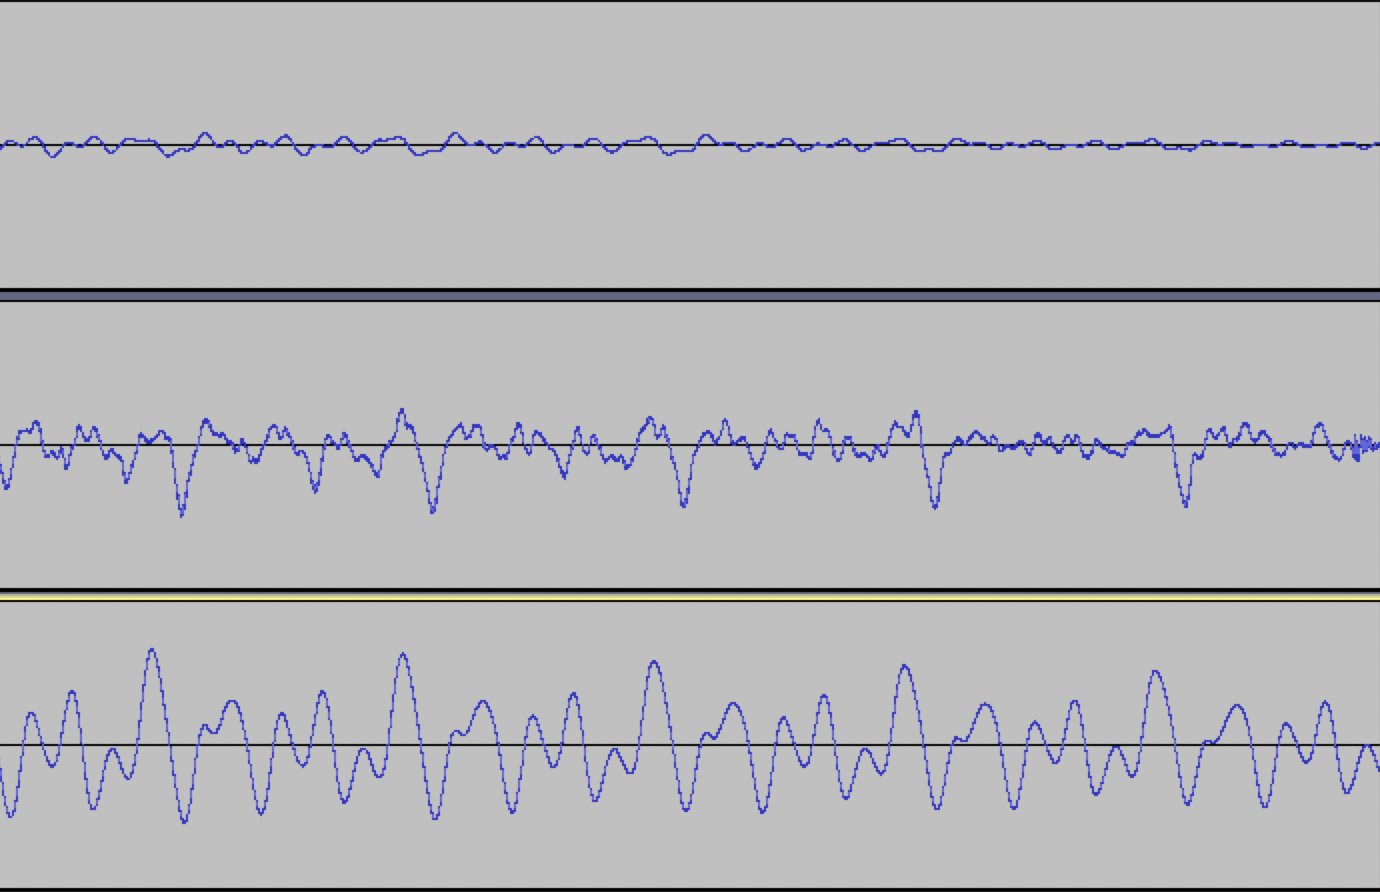
\includegraphics[height=80pt]{figure/88_88_det/a0_0800_1000.png}
\subcaption[A0の音波]{A0の0.800秒から1.000秒まで}
\label{fig:88_88_reduce1}
\end{minipage}
\begin{minipage}[b]{0.48\columnwidth}
\centering
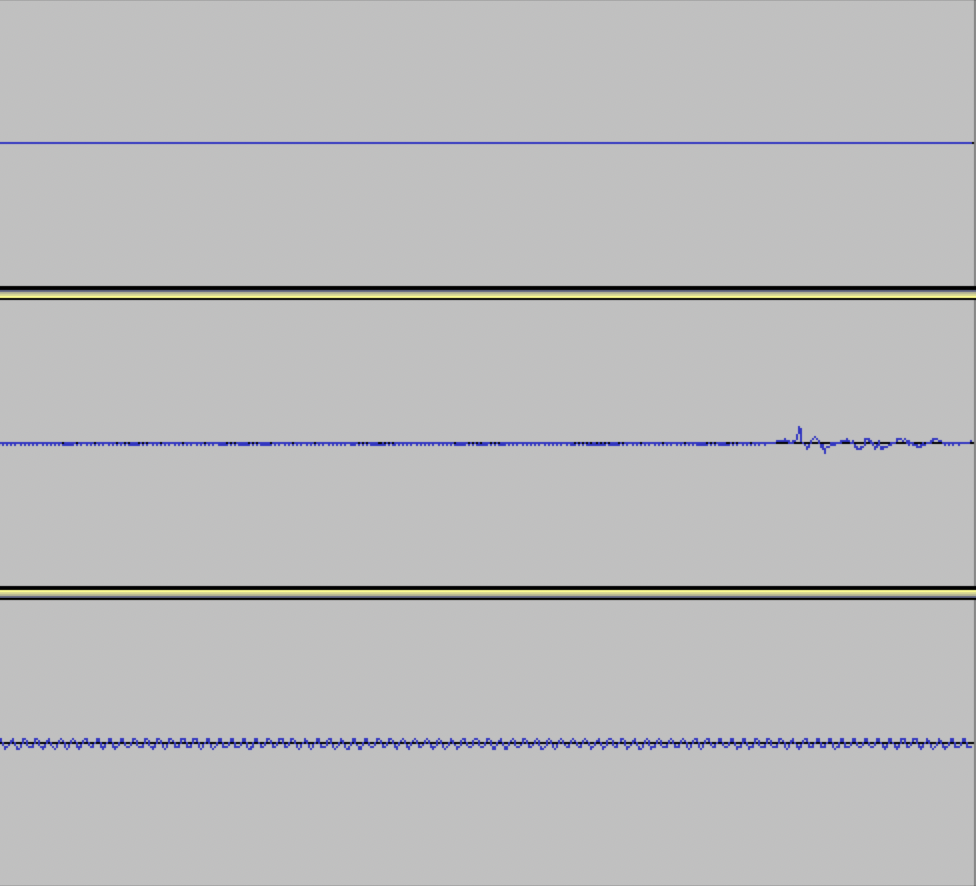
\includegraphics[height=80pt]{figure/88_88_det/b7_0980_1000.png}
\subcaption[B7の音波]{B7の0.980秒から1.000秒まで}
\label{fig:88_88_reduce2}
\end{minipage}
\caption[課題:音の減衰の表現]{}
\end{figure}

\subsubsection{音の大きさの維持}

部分的に大きさを維持できていない音がいくつかあった。特に波形の前半で生成波形の振幅が小さくなる様子が多く見られた~(\prettyref{fig:88_88_amp})~。振幅の無作為化が原因であると考えられ、学習の初段階での振幅の固定や振幅の大きさの別のネットワークによる調整などの工夫が必要であると考えられる。
    
\subsubsection{音波の滑らかさの表現}

ノイズまじりの音がいくつかあった。これらの音では音波の滑らかさを表現できていないことがわかった~(\prettyref{fig:88_88_smooth})~。音波を滑らかにするような加工を生成後に加えるなどの工夫が必要であると考えられるが、音波の滑らかさを表現できないという課題は他の音の生成の研究でも見られる。

\begin{figure}[b]
\centering
\begin{minipage}[b]{0.48\columnwidth}
\centering
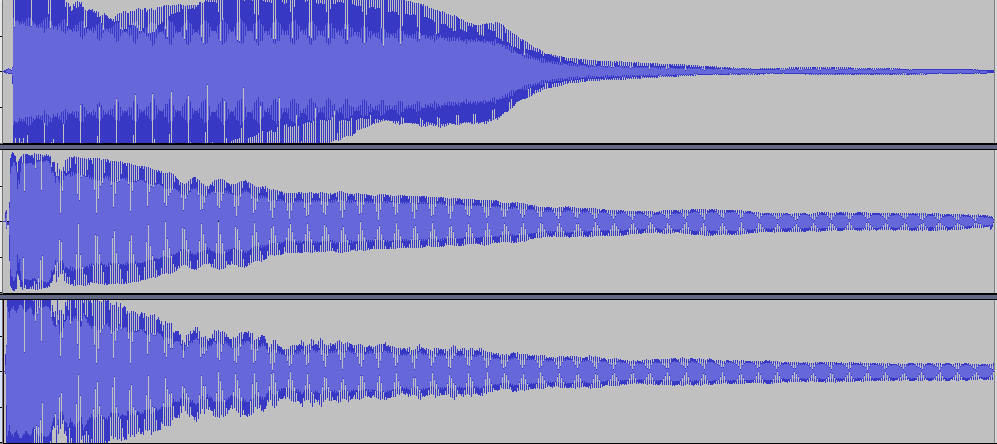
\includegraphics[height=80pt]{figure/88_88/c5.png}
\caption[課題:音の大きさの維持]{C5の0.000秒から1.000秒まで}
\label{fig:88_88_amp}
\end{minipage}
\begin{minipage}[b]{0.48\columnwidth}
\centering
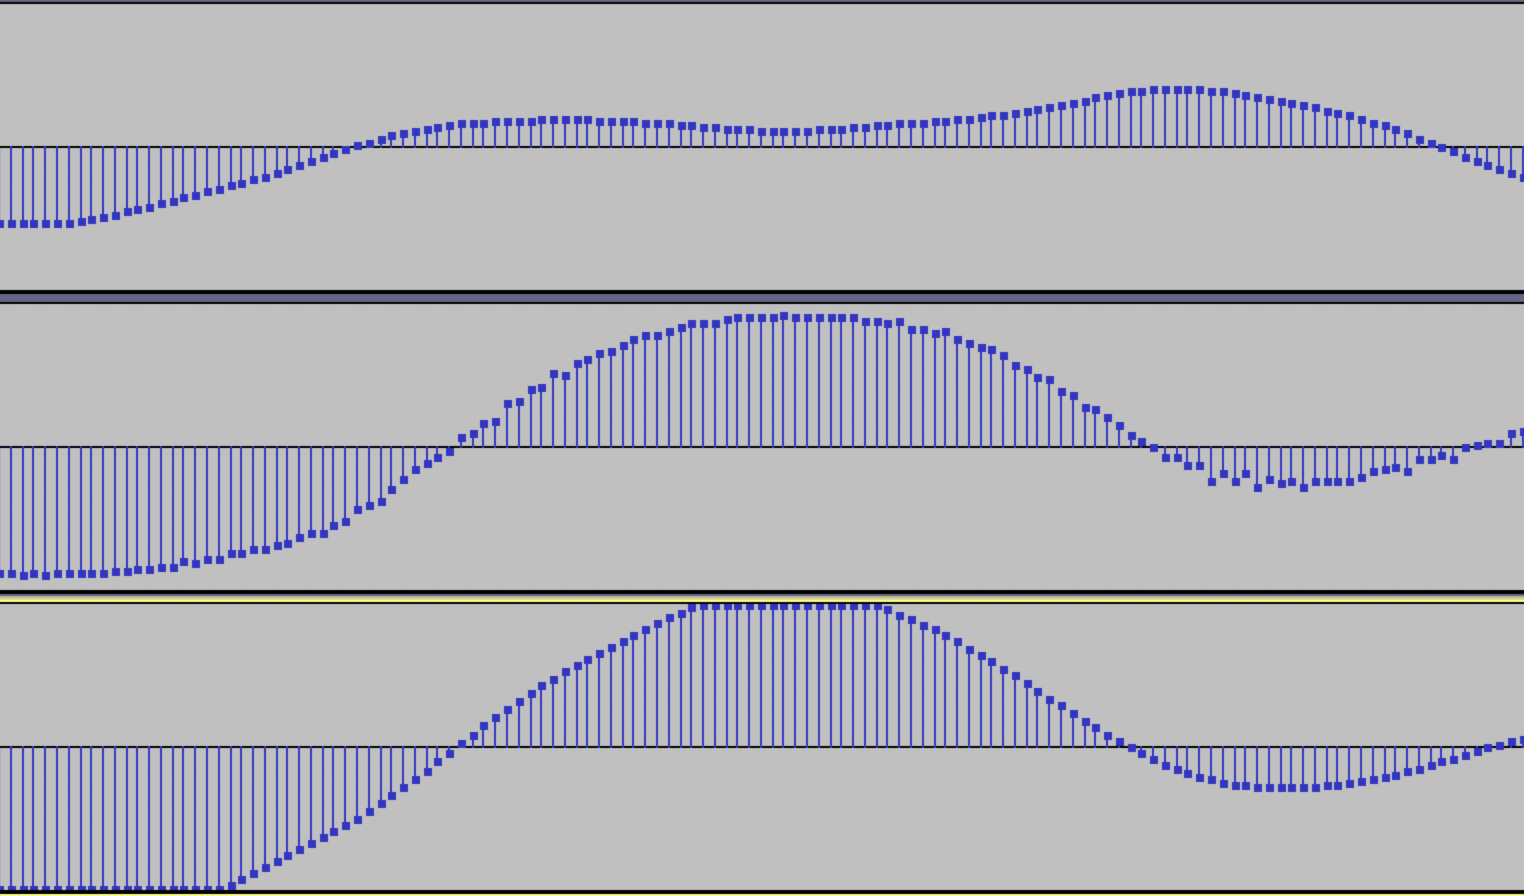
\includegraphics[height=80pt]{figure/88_88_det/d2s_0100_0103.png}
\caption[課題:音波の滑らかさの表現]{D2$\sharp$の0.100秒から0.103秒まで}
\label{fig:88_88_smooth}
\end{minipage}
\end{figure}

\subsubsection{データセットの不安定さ}

ここまでの三つは提案モデルの改善により解消されると考えられるが、問題のあるデータセットが一部に見られた。一つの問題点は高音において振動が不安定になることであり、\prettyref{sec:harp_rep}にて述べた。そして、音の鳴り出しでの振動が不安定であるという問題点も見られた。具体的には、ギターの音の鳴り出しの遅延の方がハープより大きい場合~(\prettyref{fig:88_88_lag1})~や周期的な音になるまでに遅延があるために不規則な振動となる場合~(\prettyref{fig:88_88_lag2})~などがあった。

\begin{figure}[b]
\centering
\begin{minipage}[b]{0.48\columnwidth}
\centering
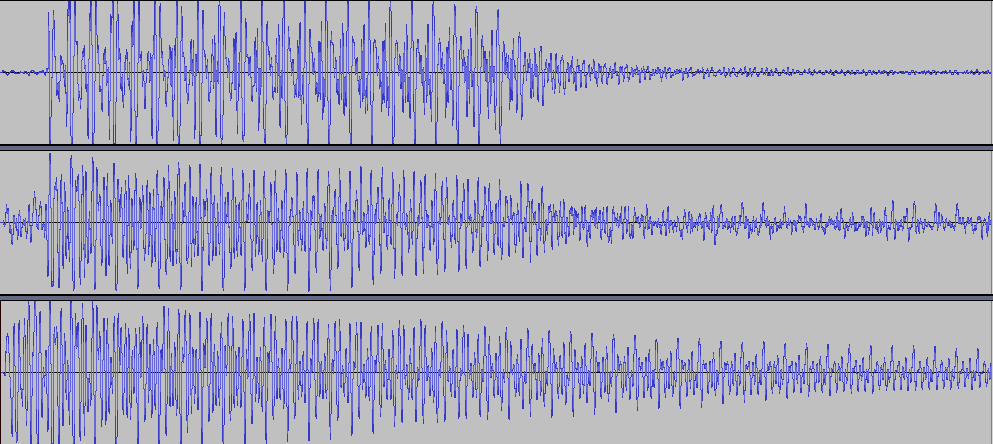
\includegraphics[height=80pt]{figure/88_88/f1s.png}
\subcaption[F1$\sharp$の音波]{F1$\sharp$の0.000秒から1.000秒まで}
\label{fig:88_88_lag1}
\end{minipage}
\begin{minipage}[b]{0.48\columnwidth}
\centering
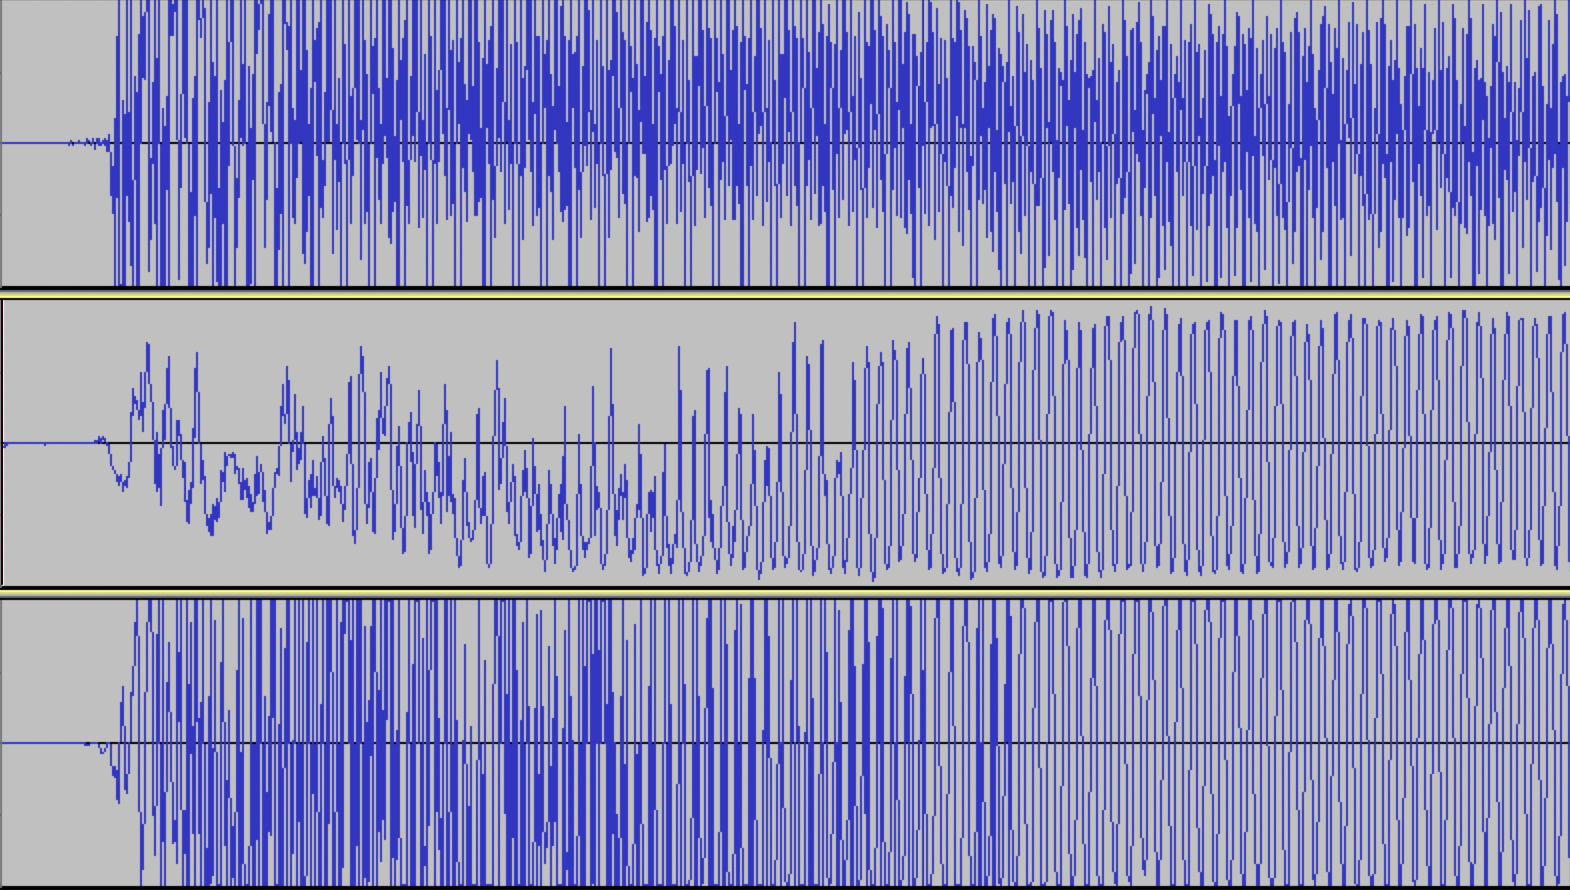
\includegraphics[height=80pt]{figure/88_88_det/a7_0_0030.png}
\subcaption[A7の音波]{A7の0.000秒から0.030秒まで}
\label{fig:88_88_lag2}
\end{minipage}
\caption[課題:データセットの不安定さ]{}
\end{figure}